%
% File acl2014.tex
%
% Contact: koller@ling.uni-potsdam.de, yusuke@nii.ac.jp
%%
%% Based on the style files for ACL-2013, which were, in turn,
%% Based on the style files for ACL-2012, which were, in turn,
%% based on the style files for ACL-2011, which were, in turn,
%% based on the style files for ACL-2010, which were, in turn,
%% based on the style files for ACL-IJCNLP-2009, which were, in turn,
%% based on the style files for EACL-2009 and IJCNLP-2008...

%% Based on the style files for EACL 2006 by
%%e.agirre@ehu.es or Sergi.Balari@uab.es
%% and that of ACL 08 by Joakim Nivre and Noah Smith

\documentclass[11pt]{article}
\usepackage[utf8]{inputenc}
\usepackage[french]{babel}
\usepackage{acl/acl2014}
\usepackage{times}
\usepackage{url}
\usepackage{latexsym}
\usepackage{graphicx}
\usepackage{natbib}
\usepackage[colorlinks=true, allcolors=blue]{hyperref}

\graphicspath{{./fig/}{.}}

\usepackage[toc,nonumberlist]{glossaries}
\AtBeginDocument{%
	\setlength\LTleft{0pt}
	\setlength\LTright{0pt}
	\setlength\glsdescwidth{0.8\hsize}
	\renewcommand{\glsnamefont}[1]{\textbf{#1}}
	\renewcommand*{\glossaryname}{Liste des symboles et abréviations}}
\makeglossaries
% \renewcommand{\acronymname}{}
\loadglsentries{gls/glossary}
\glsaddall


%\setlength\titlebox{5cm}

% You can expand the titlebox if you need extra space
% to show all the authors. Please do not make the titlebox
% smaller than 5cm (the original size); we will check this
% in the camera-ready version and ask you to change it back.


\title{Agents conversationnels à base de réseaux de neurones artificiels profonds}

\author{Guillaume Chevalier \\
  Université Laval \\ Baccalauréat en génie logiciel \\
  {\tt \small guillaume.chevalier.2@ulaval.ca} \\\And
  Samuel Cabral Cruz \\
  Université Laval \\ Baccalauréat en génie logiciel \\
  {\tt \small samuel.cabral-cruz.1@ulaval.ca}}

\date{}

\begin{document}
\maketitle

\begin{abstract}
  Les approches par réseaux de neurones ont récemment surpassées les approches par algorithmes classiques en ce qui concerne la majorité des problèmes du traitement de la langue naturelle. C'est principalement ce qui explique pourquoi nous voyons de plus en plus de solutions commerciales implémentant des agents conversationnels, tels que \textbf{Siri (Apple)}\footnote{\url{https://www.apple.com/ca/ios/siri/}}, \textbf{Alexa (Amazon)}\footnote{\url{https://developer.amazon.com/alexa}} et \textbf{Google Assistant(Google)}\footnote{\url{https://assistant.google.com/}}. \\

  Devons-nous toutefois croire que la réalisation d'un tel agent et une discipline réservée aux géants de l'industrie technologique? Comment s'y prennent-ils? Est-ce envisageable de se créer notre propre agent conversationnel? Si oui, Comment? \\

  Dans cet article, nous tenterons de répondre à chacune de ses questions en se basant sur les parutions d'études récentes. Pour ce faire, nous déquortiquerons le problème en plusieurs étapes qui devront être accomplies par notre agent conversationnel hypothétique. De cette façon, il sera beaucoup plus simple d'avoir une représentation mentale des différentes parties nécessaires à la construction d’une architecture entièrement neurale pour les agents conversationnels.
\end{abstract}

\section{Introduction}

Depuis la naissance de l'informatique, l'humain a toujours convoité l'idée de pouvoir intéragir verbalement avec un ordinateur, et ce, de manière transparente comme s'il s'agissait d'un autre humain apte à capter la majorité des nuances du discours entretenu. Les premières tentatives (\textbf{ELIZA} - \textit{the artificially-intelligent psychiatrist} \cite{elizaWeizenbaum} et   \textbf{PARRY} - \textit{the paranoid computer}1 \cite{parryCerf}) ont cependant démontré que cette tâche était loin d'être simple et qu'aucun algorithme ne pourra éventuellement répondre parfaitement à cette tâche et ainsi être considérée suffisamment intelligente pour passer le test de Turing \cite{turingTest}. Bien que ce sujet aura fait couler beaucoup d'encre et fait tourner les têtes, il n'existe toujours pas à ce jour une formule secrète parfaite pour parvenir à sa réalisation. Au cours des années, différentes démarches ont été proposées. Traditionnellement, des approches algorithmiques étaient favorisées et certains projets se fondent encore sur ces dernières, tel que \textbf{Watson (IBM)}\footnote{\url{https://www.ibm.com/watson/}} \cite{ibmWatson}. Ces approches ont toutefois le défaut d'être longues et ardues à développer. De plus, la réutilisation des travaux sous-jacents est plus complexe en raison du caractère sur-mesure du problème, en lien avec le champ d'application spécifique, tel que de jouer à \textbf{Jeopardy} \footnote{\url{https://www.jeopardy.com/}}. Depuis 2014, ce type d'approche classique fut appelé à changer par des approches fonctionnant par réseaux de neurones profonds, le point marquant de ce virage étant la découverte des mécanismes d'attention par \cite{attentionMechanism}. \\

De ce fait, des approches mettant en jeu des réseaux de neurones artificiels ont fait leur apparition et ont immédiatement connus beaucoup de succès. C'est l'apparition des mécanismes d'attention, en 2014, qui marquera un dépassement significatif des performances des techniques classiques pour la tâche de la traduction automatique \cite{attentionMechanism}. De tels systèmes sont désormais utilisés chez \textbf{Google} pour la mise en production du fameux \textbf{Google Translate} \cite{googleTranslate}, avec leur publication officielle d'une amélioration de cette architecture neurale plus tard en octobre 2016. Cette même compagnie utilise aussi des algorithmes de \gls{tts} tels que tels que celui de \cite{acousticModeling} afin de pouvoir générer des sous-titres automatiquement pour de l'audio ou des vidéos (comme \textbf{YouTube} le fait avec des recherches similaires) et afin de pouvoir analyser les vidéos et les lier entre elles avec une approche sémantique. \\

Il ne s'agit ici que de différents morceaux de puzzle complet qui peuvent mener à la création d'un agent conversationnel complètement basé sur ces systèmes par réseaux de neurones. La création d'un tel agent est une tâche compliquée dû au fait qu'il faut assembler les découvertes des différentes parties, l'une des raisons pourquoi le mouvement open-source est si proéminent. Dans le cadre d'un échange verbal entre deux êtres, une multitude de tâches sont accomplies sans même que nous ne soyons conscient. Le tout débute lors d'un contact initial le plus souvent dans une forme auditive vers un destinataire. En partant de ce point, à titre de destinataire, il faut premièrement capter le message, l'interpréter en mots et, malgré des obstacles environnants et culturels variés réduisant la qualité de cette transmission, filtrer ce qui est réellement important dans le signal ainsi que le décoder selon un dialecte particulier. C'est à cette étape que s'insère les architectures de \gls{stt}. Une fois en possession de ce message, il faut établir des liens entre l'énoncé qui a été donné et un registre de connaissances en plus de prendre en compte les discussions passées avec le même interlocuteur. C'est alors qu'il est possible d'établir la réponse la plus appropriée compte tenu d'une panoplie de facteurs comme l'identité de notre interlocuteur, son domaine de travail et son niveau d'éducation, les valeurs qui sont partagées ou distinctes entre les deux parties. Cette phase implique des réseaux de neurones capables d'analyser du texte à partir d'une requête, tels que les systèmes basés sur des améliorations et une exploration des mécanismes d'attention \cite{attentionBasedApproaches} ensuite appliquées à cette nouvelle tâche, introduits dans les travaux de \cite{readNcomprehend}. L'attention étant maintenant bien attribuée dans le texte, il est ensuite possible de générer une réponse, tel qu'avec les recherches récentes de \cite{chatbot\string:HRED} et de \cite{chatbot\string:LVHRED}.\\

Une fois cette réponse textuelle en main, il ne reste qu'à la convertir en audio, ce qui est dorénavant possible de générer en temps réel avec une approche par réseaux de neurones convolutionnels tels que \texttt{Wavenet} par \cite{wavenet} (encore une fois développé chez \textbf{Google} pour faire du \gls{tts}, l'inverse du \gls{stt}). L'un des plus grands obstacles à cela est lorsque les utilisateurs possèdent un accent fortement prononcé et qui est unique en plus d'utiliser un dialecte différent. Au moins, ce genre de systèmes est suffisamment flexible pour opérer en plusieurs langues en leur fournissant un module de traduction automatisé. Au final, cela demande beaucoup de données d'apprentissage. Pour rajouter encore plus de difficulté, ces étapes sont à faire dans un interval de temps très rapide. Heureusement, l'étape la plus longue est de faire apprendre aux réseaux de neurones ce qu'ils ont à apprendre, tâche pouvant être réalisée à priori et réutiliser à répitition une fois terminée. Ils sont ensuite très performants lors de l'étape d'inférence, où ils analyse et génèrent réellement de l'information en production. \\

\section{Développement}
Toutes les parties nécessaires pour concevoir un agent conversationnel basé sur une architecture neuronale existent présentement. Certaines techniques se sont démarquées au fil des études. Un survol rapide des techniques les plus prometteuses est fait, de façon à ce qu'il soit possible de joindre ces dernières ensemble ce qui permettrait d'en faire une implémentation réelle et complète. Les approches neuronales les plus aux goûts du jour sont à favoriser et sont introduites dans cet article. Ces approches imitent la nature et correspondent, à ce jour, à la forme la plus répandue d'intelligence artificielle. Il ne reste qu'à les informatiser convenablement et à découvrir les bonnes configurations neuronales dans le but de créer l'interface conversationnelle idéale. \\

\subsection{Traitement d'un intrant vocal}
La première étape de calcul au sein d’une architecture neurale destinée à comprendre et répondre à un utilisateur est justement de comprendre ce qu’il dit. Pour accomplir cette tâche, il est possible d’utiliser un réseaux de neurones \gls{tc}-\gls{dnn}-\gls{bilstm}-\gls{dnn}, c’est-à-dire des convolutions temporelles (TC) suivies de couches de neurones linéaires profondes (DNN), d’un LSTM Bidirectionnel (BLSTM) et puis d’un second DNN final \cite{acousticModeling}. Ainsi, cette architecture dépend d’un pré-traitement du signal par un autre algorithme lequel est plus classique et permet de transformer le signal en un domaine de fréquences personnalisées. C’est ce pré-traitement de l’information qui est introduit dans le réseau de neurones profond, afin d’en analyser le sens et de pouvoir convertir cela en états acoustiques, lesquels peuvent être convertis, cette fois, en texte littéraire. Cette architecture neurale, imagée à la \autoref{fig:tcDnnBlstmDnn}, obtient un \gls{wer} de retranscription de 3.47, ce qui est présentement le \gls{sota} sur le jeux de données et problème du \gls{wsj} eval’92.

\begin{figure*}
  \centering
  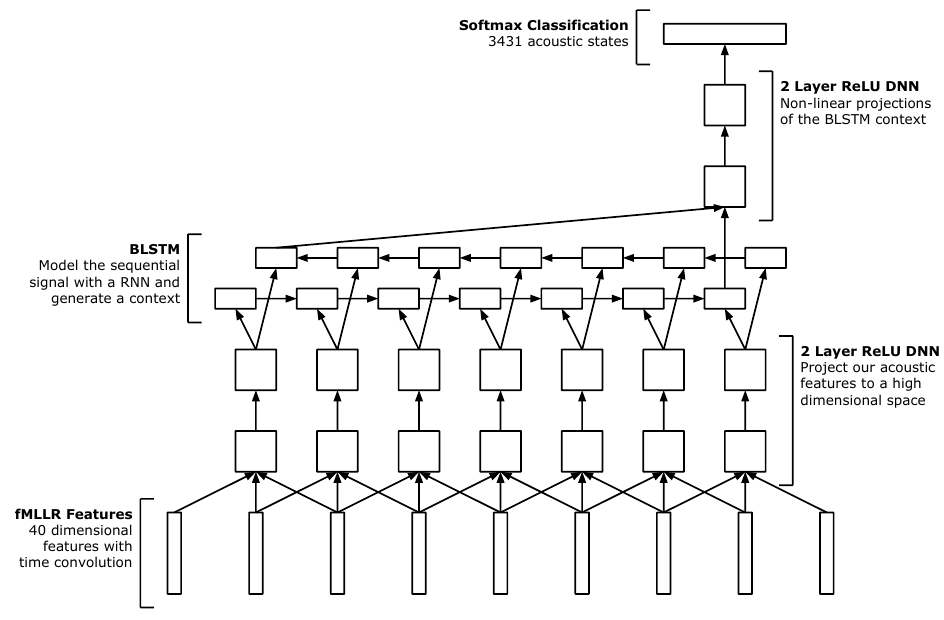
\includegraphics[width=\textwidth]{tcDnnBlstmDnn}
  \caption{L’architecture neurale \gls{tc}-\gls{dnn}-\gls{bilstm}-\gls{dnn} permet d’écouter le signal audio à l’aide des données audio extraites en \gls{fmllr}. Ainsi, un \gls{dnn} suivi d’un \gls{bilstm} peut analyser ce signal pour classifier le tout en états acoustiques, lesquels sont eux-mêmes repris par un algorithme classique qui permet de rassembler ces états en mots réels. Notons que cette architecture neural peut être utilisée pour raffiner le signal des mots prononcés, ce qui peut être envoyé directement dans un réseaux de neurones supérieur en tant que \textit{embedding}. [\citenum{acousticModeling}]}
  \label{fig:tcDnnBlstmDnn}
\end{figure*}

\subsection{Extraction des composantes de l'intrant et des sources d'information à analyser}
Une fois que la requête de l'utilisateur aura été convertie sous une forme textuelle facilement manipulable par un ordinateur, nous pourrions, dès lors, utiliser le plongement induit par l'étape précédente. Une autre approche consiste à reprendre cette sortie pour ensuite la fournir à une nouvelle structure qui se chargera d'aller extraire de nouvelles composantes qui aideront certainement à obtenir de meilleurs résultats pour la suite du processus. \\

À ce stade, nous devons comprendre que le signal est encore purement textuel et nous n'avons pour seule information qu'une décomposition des mots qui forment la demande reçue. Cependant, les langages sont formés de davantage de subtilités qu'un simple enchaînement de mots les uns après les autres. En effet, chaque mot joue un rôle précis dans la structure de la phrase et apporte une nuance particulière au contexte générale de celle-ci ou encore du texte avec une plus faible portée. C'est exactement ce que les travaux de ... visaient à faire. Ainsi, en ..., ce groupe de chercheurs a fait la publication d'un article détaillant leur approche en comparant plusieurs modèles différents comprenant autant des approches classiques que des approches neuronales. En plus de faire état de leurs travaux, ce groupe est aussi à l'origine d'outil qui est encore à ce jour considéré comme un incontournable: \cite{word2vec}. \\

Malgré le fait que cet article porte sur les approches neuronales, cet outil a plutôt prouvé que des approches plus simplistes et classiques sont parfois plus appropriées. Word2vec se fonde sur la combinaison de deux approches nommées \textit{Continuous Bag Of Words} (\autoref{fig:cbow}) et \textit{Skip-gram} (\autoref{fig:skipgram}). Alors que le \textit{Skip-gram} se concentre à essayer de prédire son contexte, le \textit{CBOW} cherchera plutôt à prédire la valeur considérée à partir de son environnement accordant ainsi plus d’importance à la structure des phrases plutôt qu’au contexte d’utilisation.\\

\begin{figure}[ht]
  \centering
  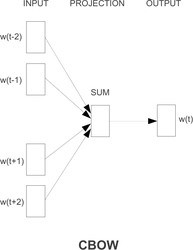
\includegraphics[width=\columnwidth, height=0.35\textheight, keepaspectratio]{cbow}
  \caption{Architecture de la méthode de prédiction CBOW [\citenum{word2vec}]}
  \label{fig:cbow}
\end{figure}

\begin{figure}[ht]
  \centering
  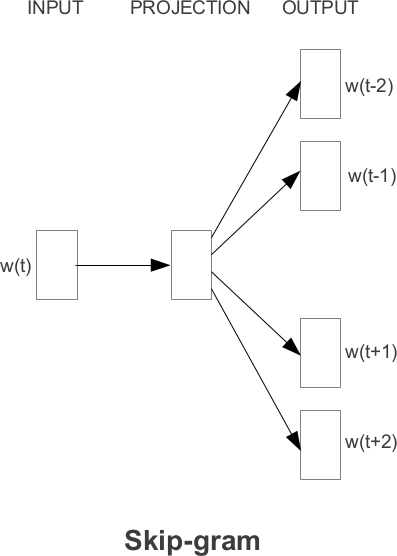
\includegraphics[width=\columnwidth, height=0.35\textheight, keepaspectratio]{skipgram}
  \caption{Architecture de la méthode de prédiction Skip-gram [\citenum{word2vec}]}
  \label{fig:skipgram}
\end{figure}

En fournissant la requête reçue à cet outil, il sera donc possible d'extraire les composantes sémantiques et syntaxiques sous-entendues par cette dernière. Par la suite, ces nouvelles composantes seront combinées à celle que nous avions déjà obtenues à l'étape précédente. En procédant avec cette seconde approche, nous réaliserons certainement un gain majeur au niveau de la performance des prochaines étapes en raison de l'ajout important de dimensionnalités qui fourniront beaucoup plus de flexibilité aux réseaux de neurones suivantes qui devront à leur tour détecter les nuances du langage. À titre d'exemple, lorsqu'un utilisateur demandera à l'assistant si ce dernier peut lui indiquer l'horaire du cinéma le plus prêt de sa position, l'assistant devra comprendre la nuance que ce qui intéresse vraiment l'utilisateur est l'horaire et non pas l'évaluation booléenne de sa capacité à s'acquitter de cette tâche. Par contre, dans le cas où l'utilisateur demanderait à l'assistant si ce dernier peut le connecté à l'Internet, l'assistant devra dans ce cas faire l'évaluation de sa capacité et répondre en par affirmation à notre cher utilisateur. \\
%TODO Référence au transfer learning

Mais qu'en est-il de nos sources d'informations? En fait, le processus entier bénéficiera certainement qu'un travail similaire soit fait à ce niveau aussi. Pour ce faire, deux approches s'offrent encore à nous. La première consistant encore une fois à utiliser word2vec et la seconde repose sur le même principe, mais à un niveau supérieur d'abstraction en considérant cette fois l'utilité de chacune des phrases dans le texte plutôt que de se concentrer sur le rôle de chaque mot dans chaque phrase \cite{inferSent}. \\

En somme, toutes ces composantes ainsi dérivée pourrons ensuite être fournies en entrée d'un réseau de neurones tel qu'un RNN tel qu'il sera expliqué à section suivante.

\subsection{Interprêter la requête et cibler le contenu d'intérêt pour y répondre}

Pour analyser les demandes de l'utilisateur, il faut les traduire en requêtes neurales pour ensuite rechercher dans le texte les passages intéressants. Cela est une étape importante à comprendre avant d'analyser d'avantage ce qui sera expliqué dans les prochaines sections. C'est l'une des choses que peuvent faire les mécanismes d'attention tels qu'introduits par Bahdanau et al. en 2014 \cite{attentionMechanism}. Ces mécanismes sont illustrés à la \autoref{fig:attn}. Son fonctionnement va comme suit. En premier lieu, le texte est lu séquentiellement en entrée (en bas à gauche). Ensuite, une requête est faite pour filtrer ce qui est lu et faire l'alignement d'attention (en bas à droite). Cette requête peut provenir d'un autre réseaux de neurones, mais est ici elle-même générée dans un contexte de traduction automatique. La requête est donc de demander par quoi la phrase devrait débuter lors de ce début de traduction, ce que le décodeur (à droite) peut utiliser pour construire mot par mot une phrase traduite avec une requête à chaque nouveau mot, séquentiellement. Cette requête est à chaque étape comparée à toute l'information à filtrer par le mécanisme d'attention (au centre). C'est ainsi qu'un résultat est formulé par ce calcul du mécanisme d'attention en fonction de la requête demandée (en haut). Les auteurs soutiennent que les mécanismes d'attention sont à explorer plus en profondeur et que cela n'est que leur début. Une certaine exploration de ce mécanisme est faite par Luong et al. en 2015 \cite{attentionBasedApproaches}. Notamment, ils définissent un tel mécanisme comme étant un mini réseaux de neurones dans un plus gros. Ce mini réseaux de neurones sert à déterminer où mettre l'attention, et peut prendre des formes variées, tel qu'un réseaux de neurones linéaire à deux couches, ou bien une comparaison par produit vectoriel de chaque élément à comparer à la requête, en tant que mesure de similarité entre la requête et les éléments d'information où rechercher.

\begin{figure*}
  \centering
  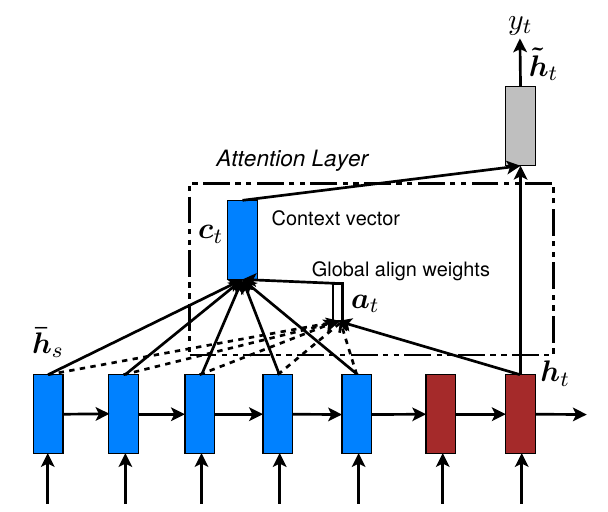
\includegraphics[width=\textwidth, height=0.4\textheight, keepaspectratio]{bahdanauAttentionMechanism2014}
  \caption{Mécanisme d'attention sous sa forme générale, tel qu'introduit par Bahdanau et al. en 2014 \cite{attentionMechanism} et ici raffinés par Luong et al \cite{attentionBasedApproaches} dans cette figure.}
  \label{fig:attn}
\end{figure*}

Il est bien d'avoir les mécanismes d'attention pour faire de la traduction automatique \cite{attentionMechanism}, mais il est tout aussi possible de les utiliser pour trouver dans du texte les passages intéressants en fonction d'une questions. C'est ce que font Cui et al. \cite{squad:attentionOverAttention}, tout comme Xiong et al. \cite{squad:coattention}, en 2016 sur le jeux de données du SQuAD \cite{squad}, cela suite aux travaux de Google de 2015 lesquels sont détaillés dans la section suivante \cite{readNcomprehend}. Les travaux de Cui et al. sont imagés à la \autoref{fig:coAttn}. La réponse est retournée suite à avoir posé une question dans le texte. Ce réseaux de neurones ressemble à celui de Google, lequel est détaillé à la section suivante. 

\begin{figure*}
  \centering
  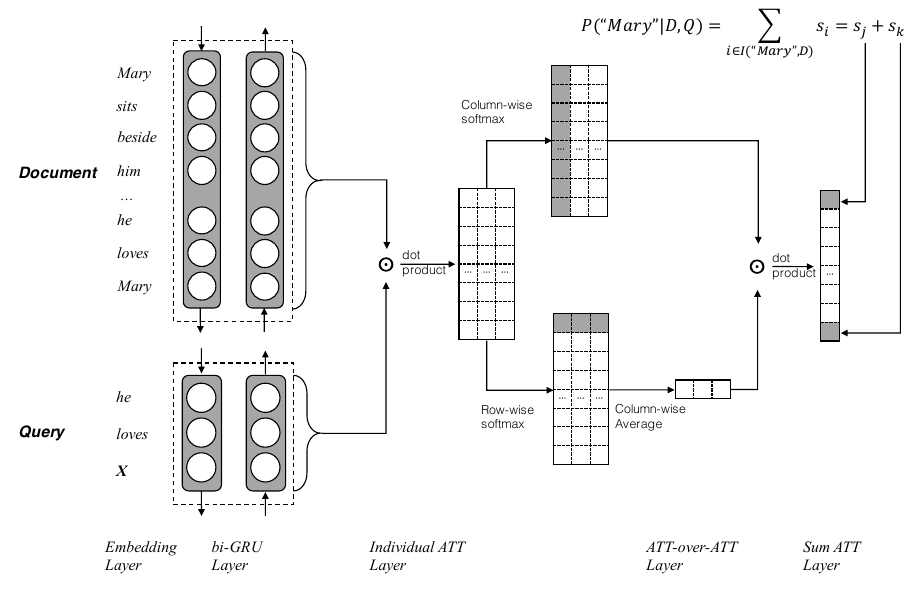
\includegraphics[width=\textwidth, height=0.4\textheight, keepaspectratio]{squadAttentionOverAttention}
  \caption{Réseaux de neurones profond permettant d'analyser un document (en haut à gauche) en fonction d'une requête (en bas à gauche) pour produire une réponse avec l'information trouvée (à droite), par Cui et al. \cite{squad:attentionOverAttention}.}
  \label{fig:coAttn}
\end{figure*}

\subsection{Formulation d'une réponse à partir de l'information d'intérêt retenue}

Bien qu’il est intéressant de trouver l’endroit où porter attention dans un corpus textuel, il est tout autant intéressant de savoir comment générer une réponse structurée et concise à l’utilisateur. Cela peut être fait en utilisant le \gls{hred} tel qu’introduit par \cite{chatbot\string:HRED}. En effet, \gls{hred} est une imbrication hiérarchique de réseaux de neurones récurrents. Un premier est utilisé afin d’encoder les phrases, un second est nécessaire afin de garder le contexte des réponses passées lesquelles ont déjà traitées, comme un suivi de la discussion dans une mémoire temporaire, et finalement un troisième \gls{rnn} est mis à profit afin de décoder l’information en une réponse à l’utilisateur. En adaptant l'architecture neurale \gls{hred} de façon à lui donner des mécanismes d'attention tels que précédemment expliqués, il est possible de générer la réponse en retour de la requête attentionnelle à l’utilisateur. Ainsi, en ayant le contexte de la question que l'utilisateur pose ainsi que le contexte des documents à parcourir avec les mécanismes d’attention, il est possible de chercher dans le texte ce qu'il faut comme information, pour faire un calcul sur cela, ce qui est envoyé au décodeur du \gls{hred} lequel peut répondre avec le nouveau contexte de l'information trouvée par la recherche effectuée. Ainsi, le premier \gls{rnn} du \gls{hred} qui encode l’information peut utiliser word2vec \cite{word2vec} directement, en plus d’utiliser un \textit{embedding} provenant de l’avant dernière couche de neurones du \gls{dnn} de \gls{stt}. En plus de cela, il est possible d’utiliser le réseau de neurones infersent de \textbf{Facebook} \cite{inferSent}, lequel peut être concaténé au signal de sortie du RNN encodeur du \gls{hred}, en tant que plongement supplémentaire au niveau des phrases plutôt qu’au niveau des mots. \\

Dans une amélioration plus récente de l’architecture \gls{hred} \cite{chatbot\string:LVHRED}, telle qu'illustré à la \autoref{fig:lvHred}, il est possible d’utiliser une variable latente intermédiaire laquelle permet de faire le pont entre les réponses envoyées du décodeur vers l’utilisateur, en plus de réinjécter cette réponse dans l’encodeur qui écoute la réponse de l’utilisateur suite à cela. En retournant ainsi l'information du du décodeur dans l’encodeur, nous nous assurons de conserver le contexte d’une phrase à la prochaine et d'ainsi avoir un discours plus fluide tout en étant moins assujettis à des variations subites de sujet ou d'interprétation. D'autre part, ce passage d'information aura pour effet de renforcer la qualité de la requête attentionnelle laquelle peut être générée à la toute fin de l’encodeur du \gls{hred}. C'est à ce moment que le mécanisme d’attention décrit dans la section précédente portant sur l’analyse de texte suite à des questions pourrait être inséré. Une fois la question posée par l’utilisateur et lue dans l’encodeur, le \gls{hred} peut bénéficier de cette question dans son \gls{rnn} intermédiaire, et ce, en tant que requête attentionnelle à passer directement au système attentionnel. Des travaux similaires ont été réalisés par \cite{readNcomprehend}, chez \textbf{Google}, lesquels sont ici inspirants. Somme toutes, le \gls{hred} aura accès à la question de l’utilisateur et au corpus de texte dans lequel il peut maintenant cibler l’information pertinente.

\begin{figure*}
  \centering
  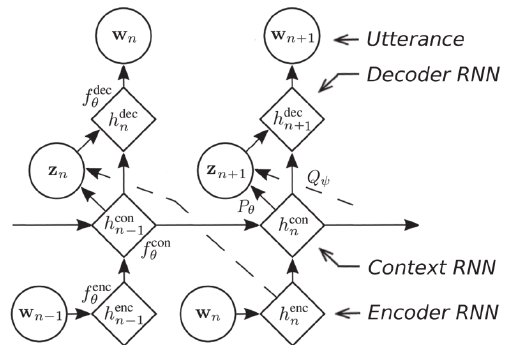
\includegraphics[width=\textwidth]{lvHred}
  \caption{L'architecture \gls{hred} améliorée avec une variable latente \cite{chatbot\string:LVHRED}}
  \label{fig:lvHred}
\end{figure*}

Étant donné la taille énorme du corpus textuel dans lequel le réseaux de neurones peut lire l’information, tel que l’ensemble du texte sur Wikipédia par exemple, il est possible d’appliquer un \texttt{MapReduce} \cite{DeanMapReduce} pour ainsi améliorer les performances de ce processus et ainsi de façon importante le temps de réponse de notre assistant, ce qui est un aspect primordial. Cette technique procède de façon distribuée sur plusieurs centaines d’ordinateurs. Dans le cas présent, ceux-ci utiliseraient eux-même les implémentations de word2vec et \texttt{inferSent} sur le corpus d'information, et cela en ayant en main la requête attentionnelle générée par le mécanisme d'attention, selon les principes de \texttt{MapReduce}. Cette partie, qui est distribuée et qui est surnommée, le lecteur impatient, est représenté à la \autoref{fig:teachingImpatientReader}. Il y a même une amélioration possible sur cet architecture neurale. Il est visible dans la figure que plusieurs itérations entre la requête et le système attentionnel est fait. Cela devrait être fait en une seule étape afin de réduire la complexité algorithmique de linéaire à constante en fonction de la longueur de la requête, en termes de nombre de mots. La recherche suite à la requête pouvant être distribuée, cela peut être fait en un temps très rapide, tout comme l'ensemble des opérations décrites dans les sections précédentes.

\begin{figure*}
  \centering
  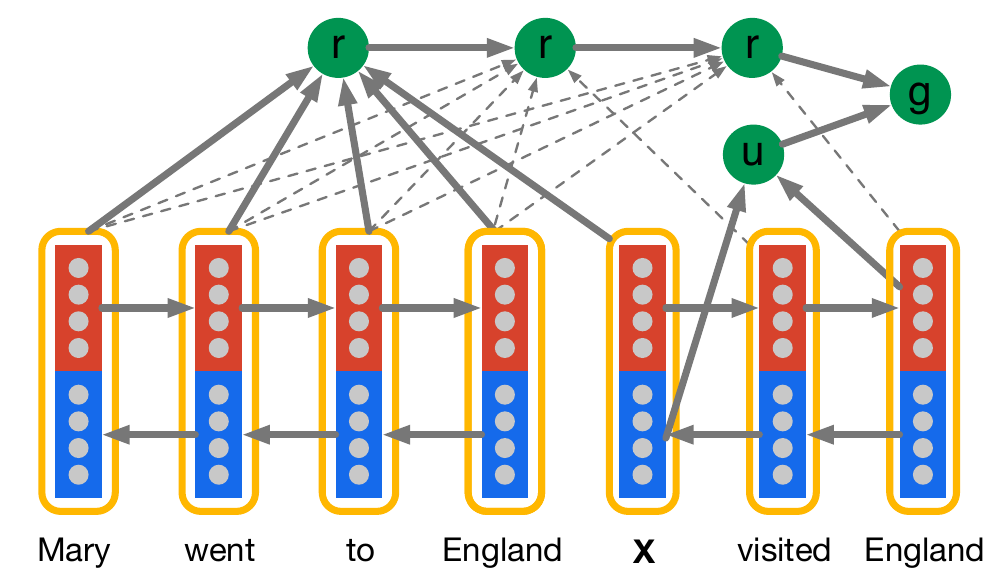
\includegraphics[width=\textwidth]{teachingImpatientReader}
  \caption{Le lecteur impatient prends la requête “X visited England” afin de faire une recherche dans le texte “Mary went to England”, à l’aide du mécanisme d’attention lequel est ici dénoté “r”, assisté de la requête “u” \cite{readNcomprehend}}
  \label{fig:teachingImpatientReader}
\end{figure*}

\subsection{Retourner la réponse textuelle sous la forme d'un signal audio}
Une fois une réponse générée, il est intéressant de générer l’audio de cette à nouveau afin de répondre à l’utilisateur, ce qui est un autre calcul rapide qui peut se faire en temps réel. Cela est possible avec le CNN (Conv.. neural net) Wavenet d’Aaron van den Oord et al., développé chez Google \cite{wavenet}. En effet, il est possible de générer n’importe quel ton de voix avec \texttt{Wavenet}, ainsi le choix de la voix de la personne qui parle peut être fait par l’utilisateur. À titre d’exemple, cette architecture neurale est tellement puissante qu’il est possible de lui faire imiter la voix du président. Cette découverte récente par Google est la première fois qu’il est possible de confondre la voix pour une voix humaine réelle plutôt qu’une voix robotique, ainsi l’illusion est bien réussie. La façon dont \texttt{Wavenet} fonctionne est d’établir un préalable statistique (une variable conditionnée) qui est donnée à un premier algorithme qui s’occupe de trouver les bons tons de voix à générer avec \texttt{Wavenet}, à partir du texte. C’est ainsi que Wavenet, conditionné lui-même par le ton de voix demandé et par le texte, peut générer la voix de façon réalistique. C’est une méthode point par point, ainsi, chaque point dans la vague audio est généré en fonction des points précédents et du conditionnement demandé, c’est très bas niveau sur le signal qui est à un taux d’échantillonage de 16 kHz lors de l’entraînement, ce qui est assez pour capturer les subtilités de quelqu’un qui parlerait réellement dans un enregistrement. Cette phase générative est illustrée dans dans la \autoref{fig:wavenet}.

\begin{figure*}
  \centering
  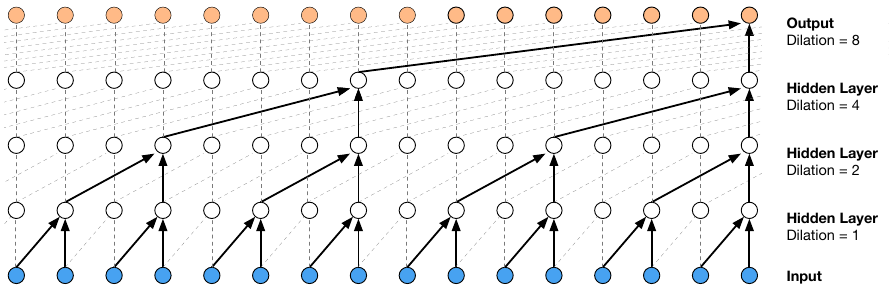
\includegraphics[width=\textwidth]{wavenet}
  \caption{À l’aide de convolutions causales dilatées, il est possible de prédire le prochain point dans la vague audio de façon efficace. Cela est un modèle autorégréssif : les points passés sont utilisés pour prédire les points suivants du même signal. Ainsi, la sortie est remise en entrée pour le calcul de l’étape suivante, ce sampling peut faire usage de mémoire cache, ce qui donne à cet algorithme générationnel un temps linéaire pour la génération, cela en fonction de la longueur du signal à générer \cite{wavenet}.}
  \label{fig:wavenet}
\end{figure*}


\section*{Conclusion}
Au terme de cet article, une revue des différentes portions d'un agent conversationnel complet a été accomplie. Nous avons introduit le sujet en abordant la conversion d'un intrant vocal sous une forme textuelle grâce à une architecture \gls{tc}-\gls{dnn}-\gls{bilstm}-\gls{dnn}. Il a aussi été mentionné que les composantes syntaxiques et sémantiques d'un texte pouvaient être extraire grâce à \texttt{word2vec} au niveau des mots ou de manière similaire avec \texttt{inferSent} au niveau des phrases. Les mécanismes d'attentions de \cite{attentionBasedApproaches}, \cite{attentionIsAllYouNeed} et \cite{attentionMechanism} pourront ensuite être exploités afin d’identifier l'information qui devra être retournée à l'utilisateur. Une fois en possession de cette information, celle-ci devra être intégrée dans une réponse textuelle complète respectant les règles de la langue utilisée dans l'échange. C'est à ce moment que l'architecture \gls{hred} entrera en jeu pour générer un discours fluide et cohérent. En dernier lieu, la génération d'un signal sonore artificiel sera déléguée à l'architecture \texttt{Wavenet}. Avec un peu de travail pour combiner tous ces sous-systèmes, un agent conversationnel performant en résultera. En guise de conclusion, nous remarquons que les approches par réseaux de neurones dominent encore une fois la majorité des autres approches auparavant exploitées. Ce qui a de plus extraordinaire avec ces derniers, c'est que des problèmes qui peuvent sembler, de prime abord, immensément complexes se révèlent à être beaucoup plus simples lorsque nous laissons les machines déterminer elles-mêmes les composantes et le traitement du signal à déduire en fonction de ces dernières via des solutions semi ou non-supervisées.

\section*{Remerciements}
Nous tenons à remercier Nadir Belkhiter, professeur agrégé à l'\gls{ul} et membre de l'\gls{oiq}, pour son support lors de la réalisation de cet article, et des ressources utiles lesquelles qu'il a mises à notre disposition.


% include your own bib file like this:
\bibliographystyle{acl/acl_natbib}
\bibliography{bib/ref}

\end{document}
